\section{Using justification reranking to provide interpretable question answering}
\label{sec-cl2017:relatedwork}

The ability of a user to understand why a question answering model chooses the answer that it does is critical both for having confidence in the model's selections as well as for diagnosing its errors.  Addressing this need, here we propose a question answering (QA) approach for standardized science exams that both identifies correct answers and produces compelling human-readable justifications for why those answers are correct. 

%\todo{summary of continuum again here}
%
%Covering the middle ground between shallow and formal representations, learning to rank methods based on tree-kernels~\citep{Moschitti:04} perform well for various QA tasks, including passage reranking, answer sentence selection, or answer extraction~\citep[inter alia]{Moschitti:07,Moschitti:11,Severyn:12,Severyn:13a,Severyn:13b,Tymoshenko:15}. 
%The key to tree kernels' success is their ability to automate feature engineering rather than having to rely on hand-crafted features, which allows them to explore a larger representation space. Further, tree kernels operate over structures that encode syntax and/or shallow semantics such as semantic role labeling~\citep{Severyn:12}, knowledge from structured databases~\citep{Tymoshenko:15}, and higher level semantic information such as question category and focus words~\citep{Severyn:13b}.
%Here, we similarly use structural features based on syntax, and enriched with additional information about how the answer candidate, the question, and the aggregated justification relate to each other.  
%A key difference between our work and methods based on tree kernels is that rather than selecting a contiguous segment of text (sentence or paragraph) our justifications are aggregated from multiple sentences, often from different documents. Because of this setup, we explore content representations that continue to use syntax, but combined with robust strategies for cross-sentence connections. Further, because our justification search space is increased considerably due to the ability to form cross-sentence justifications, we restrict our learning models to linear classifiers that learn efficiently at this scale. However, as discussed, tree kernels offer distinct advantages over linear models. We leave the adaptation of tree kernels to the problem discussed here as future work.

Our method first identifies the actual information need in a question (i.e., the focus words, or the portion of the question that is relevant to the inference needed to answer it) using psycholinguistic concreteness norms, then uses this information need to construct answer justifications by aggregating multiple sentences from different knowledge bases using syntactic and lexical information.  

Information aggregation (or fusion) is broadly defined as the assembly of knowledge from different sources, and has been used in several NLP applications, including summarization and QA.  In the context of summarization, information aggregation has been used to assemble summaries from non-contiguous text fragments~\citep[inter alia]{barzilay1999information,barzilay2005sentence}, while in QA, aggregation has been used to assemble answers to both factoid questions~\citep{pradhan2002building} and definitional questions~\citep{blair2003hybrid}.  Critical to the current work, in an in-depth open-domain QA error analysis, \citet{Moldovan:2003:PIE:763693.763694} identified a subset of questions for which information from a single source is not sufficient, and designated a separate class within their taxonomy of QA systems for those systems which were capable of performing answer fusion. Combining multiple sources, however, creates the need for context disambiguation -- an issue we tackle through the use of question and answer focus words.

Identifying question focus words, a subtask of question decomposition and identifying information needs, was found relevant for QA (especially factoid) early on~\citep[inter alia]{Harabagiu:00,Moldovan:2003:PIE:763693.763694} mainly as a means to identify answer types (e.g., "What is the {\em capital} of France?" indicates the expected answer type is \emph{City}).  
Recently, \citet{Park:2015} have used focus words to reduce semantic drift in query expansion, by conditioning on the focus words when expanding non-focus query words.
Similarly, here, we use focus words (from both question and answer) to reduce the interference of noise in both building and ranking answer justifications.  By identifying which words are most likely to be important for finding the answer, we are able to generate justifications that preferentially connect sentences together on these focus words.  This results in justifications that are better able to remain on-context, and as we demonstrate in Section \ref{sec-cl2017:experiments}, this boosts overall performance. 

Once the candidate answer justifications are assembled, our method selects the answer which corresponds to the best (i.e., highest-scoring) justification.  We learn which justifications are indicative of a correct answer by extending ranking perceptrons~\citep{Shen:Joshi:2005}, which have been previously used in QA~\citep{Surdeanu:11}, to include a latent layer that models the correctness of the justifications. Latent-variable perceptrons have been proposed for several other NLP tasks~\citep{liang2006end,zettlemoyer2007online,sun2009latent,hoffmann2011knowledge,fernandes2012latent,bjorkelund2014learning}, but to our knowledge, we are the first to adapt them to reranking scenarios. 

\subsection{Chapter Outline}

The remainder of this chapter is organized in the following way.  Section \ref{sec-cl2017:approach} describes our approach and how the various components of our system work together.  Section \ref{sec-cl2017:focuswords} shows how we identify the portions of the question and answer that are relevant for preforming the necessary inference -- the focus words.  Then in Section \ref{sec-cl2017:tag} we explain how we aggregate sentences from various sources to form our intersentence answer justifications.  In Section \ref{sec-cl2017:scoring} we detail the features extracted from these justifications that are used in our machine learning framework, which in turn is formally described in Section \ref{sec-cl2017:perceptron}.  
%We then rank both answers and their justifications using a reranking perceptron that treats justification quality as a latent variable.  
Then, in Section \ref{sec-cl2017:experiments} we evaluate our method on 1,000 multiple-choice questions from elementary school science exams, and empirically demonstrate that it performs better than several strong baselines.%, including neural network approaches. 
Our best configuration answers 44\% of the questions correctly, where the top justifications for 57\% of these correct answers contain a compelling human-readable justification that explains the inference required to arrive at the correct answer.  
The discussion of these results is provided in Section \ref{sec-cl2017:discussion}, then in Section \ref{sec-cl2017:erroranalysis}
we include a detailed error analysis that characterizes the justification quality for both our method and a strong baseline, and show that information aggregation is key to addressing the information need in complex questions.  Finally, we provide conclusions and future directions in Section \ref{sec-cl2017:conclusion}


%\remove{Finally, we round out our discussion of question answering systems with a comparison to the famous Watson QA system, which achieved performance on par with the human champions in the Jeopardy! game~\citep{Ferucci:12}.
%Several of the ideas proposed in our work are reminiscent of Watson. 
%For example, our component that generates text aggregation graphs (Section 5) shares functionality with the Prismatic engine used in Watson. Similar to Watson, we extract evidence from multiple knowledge bases. However, there are three fundamental differences between Watson and this work. 
%First, while Watson includes components for evidence gathering and scoring (we call these justifications), it uses a fundamentally different strategy for evidence generation. Similar to most previous work, the textual evidence extracted by Watson always takes the form of a contiguous segment of text~\citep{murdock2012textual},\footnote{Watson also generates ``structured evidence'' which is obtained by converting texts to structured representations similar to logic forms, which are then matched against structured databases for answer extraction. However, this ``logical representation of a clue and then finding the identical representation'' in a database resulted in ``confident answers less than 2\% of the time''~\citep{Ferucci:12}.} whereas our justifications aggregate texts from different documents or knowledge bases. We demonstrate in this work that information aggregation from multiple knowledge bases is fundamental for answering the science exam questions that are our focus (Section 8). 
%Second, our answer ranking approach jointly ranks candidate answers and their justifications using a latent-variable learning algorithm, whereas Watson follows a pipeline approach where first evidence is generated, then answers are ranked~\citep{gondek2012framework}. We show in Section 8 that jointly learning answers and their justifications is beneficial. 
%Last but not least, Watson was implemented as a combination of distinct models triggered by the different types of Jeopardy! questions, whereas our approach deploys a single model for all questions. Our analysis in Section~\ref{sec-cl2017:erroranalysis} suggests that there are limits to our simple approach: we measure a ceiling performance for our single-model approach of approximately 70\%. To surpass this ceiling, one would have to  implemented dedicated domain-specific methods for the difficult problems left unsolved by our approach. }




\section{Approach}
\label{sec-cl2017:approach}

\begin{figure}[t!]
\centering

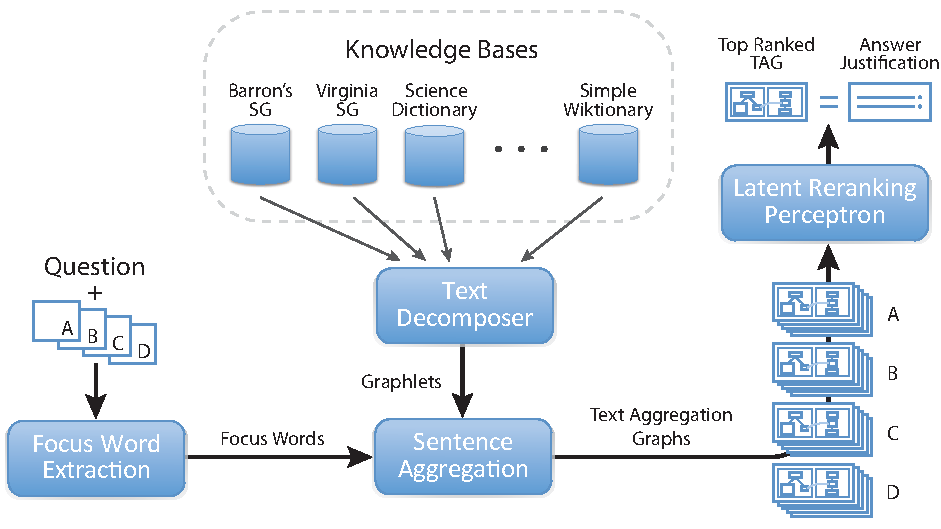
\includegraphics[width=1.0\textwidth]{mainmatter/tacl2015-tig/tag_architecture6c.pdf}

%space{-2mm}
\caption{Our QA approach, which centers on the construction of answer justifications as text aggregation graphs, and ranking them using a model that treats the justification quality as a latent variable.}
%space{-2mm}
\label{fig:architecture}
%\end{center}
\end{figure}

The architecture of our proposed QA approach is illustrated in Figure~\ref{fig:architecture}, and proceeds in a stage-like fashion.  

Prior to the QA task, in an offline process, we decompose sentences from six corpora into a lightly-structured graphical representation ("graphlets") that splits sentences on clausal and prepositional boundaries (Section~\ref{sec-cl2017:tag}). As shown later, this is fundamental to the creation and evaluation of answer justifications.  All other stages of the framework occur online. 

The QA pipeline receives as input questions with multiple choice answers, similar to the questions shown in Table~\ref{tab:inferenceexamples}, and proceeds as follows. First, the questions are fed into a focus word extractor (Section \ref{sec-cl2017:focuswords}) that produces a weighted list of the keywords from both the question and answer candidates, sorted in descending order of their likely relevance to the information needed in the question. These keywords are used by the sentence aggregation component (Section \ref{sec-cl2017:tag}) to create an exhaustive list of potential answer justifications, for each answer candidate.  These answer justifications are in the form of text aggregation graphs (TAGs), each composed of two to three graphlets produced by the above preprocessing step.

After the sentence aggregation step, each of the multiple choice answers has a long list of candidate justifications.  Because of the large number of candidate justifications created for each question/answer pair (typically tens or hundreds of thousands), we filter the list to include only the top $k$ justifications based on an inexpensive score, implemented as the sum of the weights of the focus words present in each justification\footnote{We keep ties in this filtered list, which, due to the simplicity of the score, may increase the size of the filtered lists considerably. For example, if $k=25$, it is common that the filtered list includes between $100$ and $1,000$ candidate justifications.}. 
Using the focus words, we extract a number of features from each candidate justification that measure how well the justification answers the question (Section ~\ref{sec-cl2017:scoring}), and present this information to a latent-variable perceptron ranker (Section~\ref{sec-cl2017:perceptron}).  This learning framework learns which answer candidate is correct based on the candidate justifications, while also jointly learning to rank justification quality as a latent variable, selectively elevating good answer justifications to the top of the list.  

The candidate answer with the highest-scoring justification is taken to be the correct answer.  While the justification is expressed in the form of a text aggregation graph to make it easier to assemble and evaluate, we use the original sentences from the knowledge base used to construct that text aggregation graph as a human-readable justification for why that answer candidate is correct. 
